\documentclass{article}
\usepackage{amsfonts}
\usepackage{amsthm}
\usepackage{amsmath}
\usepackage{graphicx}
\usepackage{listings}
\usepackage{hyperref}
\bibliographystyle{IEEEtran}
\setlength{\parindent}{0cm}
\lstset{
    numbers=left,
    numbersep=15pt,
    numberfirstline = false,
    breaklines=true,
}
\begin{document}

\title{Tercer Problema DAA}
\author{Karlos Alejandro Alfonso Rodríguez \\ Karel Camilo Manresa Leon}
\maketitle
\newpage

\section*{Problema}
    
    La Pregunta
    Estaba Karlos pasando (tal vez perdiendo) el tiempo cuando viene Karel y le
    hace una pregunta. Karlos quería responder que "no" a la pregunta, pero
    Karel le dijo que no era tan fácil, que la respuesta a esa pregunta iba a
    depender de un conjunto de pequeñas preguntas de "si" o "no" que este
    tenía. Luego, con las respuestas a esas preguntas de "si" o "no" armó una
    expresión booleana conformada por negaciones, expresiones "and",
    expresiones "or" e implicaciones de las pequeñas preguntas. La respuesta
    de la pregunta grande dependería de la expresión booleana que a la vez
    dependía de las pequeñas preguntas. Ayude a Karlos a encontrar si existe
    una distribución de respuestas a las pequeñas preguntas que le permitan
    responder que "no" a la pregunta grande.

\section*{Problema en términos matemáticos}

    Dada una expresión booleana, se quiere saber para que asignación de las variables
    la expresión evalúa $False$. 

\section*{Análisis del problema}

    Sea $P^*$ el problema \textbf{La Pregunta}, dicho problema es de optimización, ya que pide buscar 
    una distribución de valores para las variables de la expresión booleana. Sea $P$ la versión de decisión
    de $P^*$, es decir, se quiere saber si existe una alguna distribución de valores para las variables de la expresión
    tal que dicha expresión evalúe $False$. Demostremos que $P$ es $NP-completo$, luego $P^*$ será $NP-Hard$.

    \subsection*{NP-completitud de P}
        \subsubsection*{NP}

            Sea $A$ un algoritmo que puede verificar $P$. Una de las entradas de $A$ es una 
            codificación estándar de una fórmula lógica $F$ (literales, negaciones, expresiones and, 
            expresiones or, implicaciones). La otra entrada es un certificado correspondiente 
            a una asignación de un valor booleano a cada una de las variables de la fórmula $F$. 

            El algoritmo $A$ se construye de la siguiente manera. Se genera una $FNC$ de $\urcorner F$, luego por 
            cada cláusula de $FNC$ se verifica el valor de sus literales en la asignación. 
            Si una cláusula $C$ contiene al menos un literal que 
            su asignación sea positiva, entonces dicha cláusula será positiva, en caso de que todos los literales
            de $C$ tengan asignaciones negativos, entonces $C$ será negativa. Si todas las cláusulas de $FNC$ 
            son positivas, entonces $FNC$ será positiva; en caso contrario $FNC$ será negativa. La respuesta de $A$
            será la satisfacibilidad de $FNC$. 

            Generar la $FNC$ de $\urcorner F$ se realiza en tiempo polinomial utilizando el algoritmo de Tseitin \cite{Tseitin1970}. 
            Luego 
            el recorrido por cada cláusula y cada literal se realiza en $O(|cnf|)$, donde
            $cnf$ es la forma normal conjuntiva de la fórmula inicial, por lo tanto $A$ es polinomial. 
            Luego el algoritmo $A$ tiene tiempo polinomial. Luego $P$ es $NP$.

        \subsubsection*{Reducción}

            Se seleccionó el problema $NP-completo$ SAT (Boolean satisfiability problem) como problema conocido para 
            aplicarle una reducción polinómica al problema $P$.
            
            El problema SAT, tiene como entrada una expresión lógica en forma normal conjuntiva ($FNC$). El problema $P$, 
            tiene como entrada una expresión lógica cualquiera $F$, podemos transformar $F$ en una entrada de SAT 
            (en tiempo polinomial) aplicando el algoritmo de Tseitin sobre $\urcorner F$. 
            Entonces $FNC$ será la entrada de SAT.
            
            Sea $S$ una salida del problema SAT, $S$ será la salida correcta de $P$, ya que como $FNC \cong \urcorner F$, entonces 
            $FNC = True \Rightarrow  F = False$ y $FNC = False \Rightarrow F = True$. Luego $S$ soluciona el problema $P$.

        \subsubsection*{Algoritmo de Tseitin}
            El algoritmo de Tseitin se basa en la introducción de variables adicionales para representar 
            subfórmulas de la fórmula original. La idea es reemplazar cada subfórmula de la fórmula original 
            con una nueva variable, y luego agregar cláusulas que relacionen estas nuevas variables con las 
            variables originales. Este proceso se repite recursivamente hasta que toda la fórmula original se ha 
            reemplazado por variables nuevas.

            Por ejemplo, consideremos la fórmula lógica $F = (p \Rightarrow q) \wedge (r \Rightarrow s)$.
            Primero, se introducen dos variables nuevas, $A$ y $B$, para representar las subfórmulas $(p \Rightarrow q)$
            y $(r \Rightarrow s)$, respectivamente. Luego, se agregan cláusulas que relacionan estas nuevas 
            variables con las variables originales: 
            \begin{itemize}
                \item $A \vee \urcorner p \vee q$
                \item $B \vee \urcorner r \vee s$
                \item $F \equiv A \wedge B$
            \end{itemize}

            En estas cláusulas, la primera y sengunda cláusula representan las implicaciones
            $(p \Rightarrow q)$ y $(r \Rightarrow s)$ como disyunciones de literales, y la tercera
            cláusula establece que la fórmula $F$ es equivalente a la conjunción de las variables nuevas
            $A$ y $B$. 

            Este algoritmo se puede aplicar de manera recursiva a las subfórmulas $A$ y $B$, si es necesario.
            El resultado final es una fórmula en $FNC$ que es lógicamente equivalente a la fórmula original.
    
\section*{Soluciones para el problema}

    Podemos clasificar el problema en dos casos según el número 
    de literales por cláusula. Si cada cláusula tiene a lo sumo dos literales, es una variante de 2-SAT. 
    En este caso, el problema puede resolverse eficientemente en tiempo polinomial.

    Por otro lado, si cada cláusula contiene tres o más literales, la complejidad del problema 
    aumenta significativamente y solo se podrá resolver en tiempo exponencial.

    \subsection*{Fuerza bruta}

        La solución más sencilla para el problema es la fuerza bruta. En este caso, se evalúa 
        cada posible asignación de valores a las variables de la expresión y se verifica si la 
        expresión es verdadera o falsa. Si la expresión es verdadera, se devuelve la asignación 
        de valores que la hace verdadera. En caso contrario, se devuelve que la expresión no es 
        satisfacible.

        \subsubsection*{Pseudocódigo}

            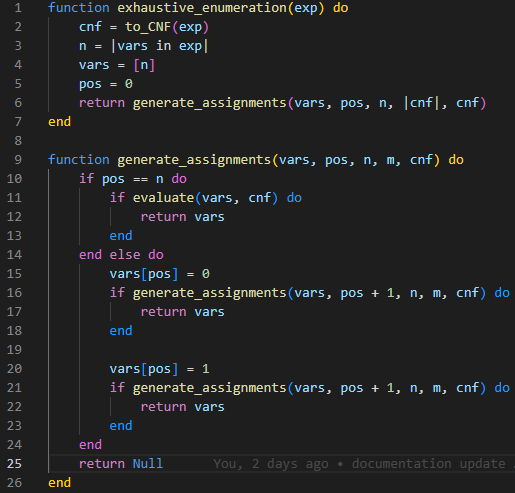
\includegraphics[width = 0.7\textwidth]{resources/code1.png}

            El algoritmo de fuerza bruta tiene una complejidad exponencial en el peor caso. En 
            particular, si la fórmula tiene $n$ variables y $m$ cláusulas, entonces el número
            de posibles asignaciones de valores de verdad es $2^n$, lo que significa que se necesitan 
            $2^n$ iteraciones para evaluar todas las posibles asignaciones. En cada iteración, el 
            algoritmo debe evaluar la fórmula lógica para determinar si la asignación actual satisface la 
            fórmula, esto implica recorrer todos los literales de cada cláusula, para 
            verificar si dicha asignación satisface la fórmula. Luego la complejidad temporal 
            sería $O(2^n * |F|)$.
    
    \subsection*{Algoritmo DPLL}
        El algoritmo DPLL (Davis-Putnam-Logemann-Loveland) es un algoritmo de resolución de satisfacibilidad booleana (SAT) que se utiliza 
        para determinar si una fórmula lógica proposicional es satisfacible.Este algoritmo trabaja de manera recursiva, y se basa en 
        la siguiente idea: si una fórmula lógica es satisfacible, 
        entonces debe ser posible encontrar una asignación de valores de verdad a las variables proposicionales que satisfaga la fórmula. 
        Por lo tanto, el algoritmo DPLL busca una asignación de valores de verdad que satisfaga la fórmula, y utiliza técnicas de poda para 
        reducir el espacio de búsqueda.
            
        El algoritmo DPLL comienza con una fórmula lógica en forma CNF, y utiliza dos tipos de reglas para simplificar la fórmula:
            
        \begin{itemize}
            \item Regla de unidad: Si una cláusula contiene solo un literal, entonces ese literal debe ser verdadero para 
            satisfacer la cláusula. Por lo tanto, se puede asignar un valor de verdad a esa variable proposicional y eliminar 
            todas las cláusulas que contienen ese literal.

            \item Regla de purga: Si una variable proposicional aparece solo en una polaridad en todas las cláusulas restantes, 
            entonces se puede asignar un valor de verdad a esa variable de manera que satisfaga todas las cláusulas que contienen 
            esa polaridad. Luego, se pueden eliminar todas las cláusulas que contienen esa variable.
        \end{itemize}

        Después de aplicar estas reglas, el algoritmo DPLL verifica si la fórmula se ha simplificado lo suficiente como para que sea 
        trivialmente satisfacible o insatisfacible.  

        Si ninguna de las reglas anteriores se puede aplicar, entonces el algoritmo DPLL elige una variable proposicional 
        arbitraria y prueba dos casos diferentes: asignarle un valor de verdad verdadero y un valor de verdad falso.
        Luego, el algoritmo DPLL aplica recursivamente las reglas de simplificación a la fórmula resultante en cada caso. 
        Si alguna de las ramas recursivas devuelve una solución satisfactoria, entonces el algoritmo DPLL devuelve esa solución.
        Si ambas devuelven contradicciones, entonces es insatisfacible.

            \subsubsection*{Pseudocódigo}
                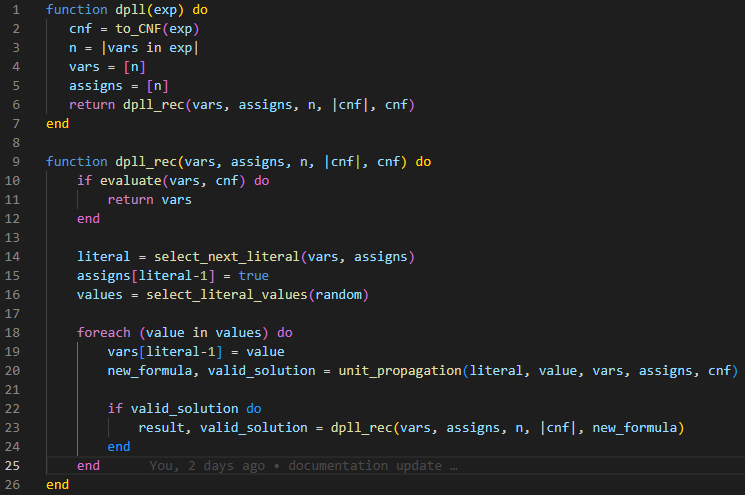
\includegraphics[width = 0.7\textwidth]{resources/code2.png}

                Métodos utilizados:
                \begin{itemize}
                    \item \textbf{select\_next\_literal:} Selecciona el proximo literal al que se le va a asignar un valor. En este caso se selecciono
                    dicho literal de manera aleatoria. No obstante existen heurísticas más complejas para esta selección que aprovechan la cantidad de 
                    variables y particularidades de la fórmula, obteniendo resultados con mayor velocidad.
                    \item \textbf{select\_literal\_values:} Selecciona el valor que tomará el literal, al igual que el método
                     \textbf{select\_next\_literal} lo hace de manera aleatoria.
                    \item \textbf{unit\_propagation:} Dado el valor y la varible seleccionados, evalúa dicha asignación y la propaga por la fórmula, 
                    verificando asignaciones triviales.
                \end{itemize}

                La complejidad temporal del algoritmo DPLL depende del tamaño de la fórmula booleana, es decir, del 
                número de variables y de cláusulas en la fórmula. En el peor caso, el número total de posibles asignaciones de 
                valores de verdad a las variables es $2^n$ ($n=cantidad\_variables$). Además las operaciones de simplificación
                (reglas de purga y unidad) se aplican por cada cláusula por tanto esto influye también en la complejidad temporal
                del algoritmo, siendo esta $O(2^n*m)$.

                Obsérvese que DPLL tiene la misma complejidad temporal que el algoritmo por fuerza bruta; no obstante, en la práctica 
                DPLL es significativamente más eficiente que la fuerza bruta debido a las técnicas de poda que utiliza (reglas de purga y unidad).
    
    \subsection*{Algoritmo genético}
        
        En el contexto del problema SAT, los algoritmos genéticos pueden ser útiles para encontrar
        una solución satisfactoria al problema. A diferencia de los algoritmos de backtracking y los algoritmos
        basados en DPLL, los algoritmos genéticos no garantizan encontrar una solución óptima 
        al problema SAT. Sin embargo, pueden ser útiles en casos donde la fórmula FNC es muy grande o compleja
        y se requiere de una solución satisfactoria en un tiempo razonable.

        El algoritmo genético implementado recibe una fórmula en FNC como entrada y sigue los siguientes pasos:

        \begin{enumerate}
            \item Representación de cromosomas:  Cada posible asignación de valores de verdad a las 
            variables proposicionales en la fórmula CNF se representa como un cromosoma. 
            En una representación binaria, cada cromosoma puede ser una cadena de bits, donde cada bit 
            representa el valor de verdad de una variable proposicional.
            \item Evaluación de la aptitud: La calidad de cada cromosoma se evalúa utilizando una 
            función de fitness que mide la satisfacibilidad de la fórmula CNF para esa 
            asignación de valores de verdad. Esta función devuelve un valor de aptitud que 
            indica el número de cláusulas que se satisfacen para esa asignación de valores de verdad.
            \item Creación de la población inicial: Se crea una población inicial de cromosomas aleatorios, 
            donde cada cromosoma representa una posible asignación de valores de verdad a 
            las variables proposicionales.
            \item Selección: Se seleccionan los cromosomas más aptos (mayor fitness) de la población actual para la 
            reproducción. Se seleccionan los $\frac{n}{2}$ mejores cromosomas como parte de la nueva población y 
            para generar $\frac{n}{2}$ nuevos cromosomas. 
            \item Operador de cruce: Se combinan dos cromosomas para producir 
            un nuevo cromosoma que comparta características de ambos progenitores.
            \item Operador de mutación: Se aplica el operador de mutación (con una probabilidad definida al inicio del algoritmo) 
            a los nuevos cromosomas 
            generados para introducir variabilidad en la población. El operador de mutación cambia 
            aleatoriamente uno o más bits en el cromosoma.
            \item Evaluación de la aptitud: Se evalúa la aptitud de los nuevos cromosomas utilizando 
            la función de fitness.
            \item Sustitución: Se sustituyen los cromosomas menos aptos de la población actual con 
            los nuevos cromosomas generados.
            \item Comprobación de la condición de terminación: Se comprueba si se ha encontrado una 
            solución satisfactoria o si se ha alcanzado un número de generaciones. 
            Si se ha encontrado una solución satisfactoria, se devuelve el mejor cromosoma como solución.
            \item Repetición del proceso: Si no se ha encontrado una solución satisfactoria, 
            se repiten los pasos 4 a 9 hasta que se cumpla la condición de terminación.
        \end{enumerate}
        
        \subsubsection*{Pseudocódigo}
            
            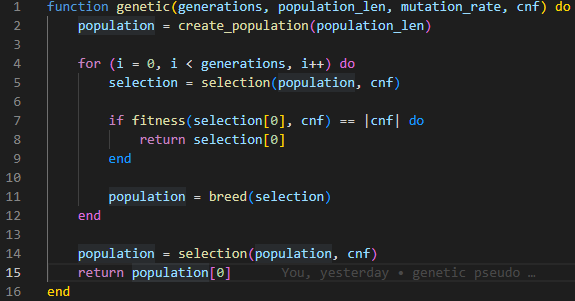
\includegraphics[width = 0.7\textwidth]{resources/code3.png}

            Para mayor comodidad, digámosle $n$ al tamaño de la población, $v$ a la cantidad de variables de 
            la fórmula, $g$ a la cantidad de generaciones del algoritmo y $l$ a la cantidad de cromosomas restantes 
            luego de seleccionar los mejores.
            
            En la complejidad temporal de este algoritmo genético influyen directamente varios procesos:
            \begin{enumerate}
                \item Generar población inicial: se crean $n$ cromosomas de tamaño $v$ de manera 
                aleatoria, por lo que la complejidad temporal sería $O(nv)$.  
                \item Simular generaciones: en la simulación de las generaciones se tienen en cuenta los siguientes
                procesos:
                    \begin{itemize}
                        \item Seleccionar mejores cromosomas: para seleccionar los mejores cromosomas, se aplica la 
                        función fitness sobre cada uno. La función fitness tiene costo $O(|cnf|)$, ya que 
                        recorre la fórmula para evaluar el cromosoma en ella. Esto se realiza por cada cromosoma, 
                        por lo que el costo de seleccionar sería $O(n|cnf|)$.  
                        \item Cruzar cromosomas seleccionados: para cruzar cromosomas se recorre la selección anterior
                        y se mezclan los cromosomas. El proceso de mezcla tiene costo $O(v)$, por lo que este 
                        proceso tiene complejidad $O(lv) \leq O(nv)$. 
                        \item Ciclo: los procesos anteriores se ejecutan $g$ veces. Por tanto 
                        este ciclo tiene costo $O(gn(|cnf|+v))$. Como $v \leq |cnf|$,
                        entonces la complejidad sería $O(gn|cnf|)$.
                    \end{itemize}
                \item Selección final: para la selección del cromosoma final se realiza nuevamente el proceso 
                de selección, con costo $O(n|cnf|)$.
            \end{enumerate}

            Tras el análisis anterior se puede determinar que el costo total del algoritmo genético es $O(gn|cnf|)$. 
    
    \subsection*{Algoritmo 2-Sat}
        
        Uno de los casos particulares del problema SAT, es el problema 2-SAT (solamente dos variables por cada cláusula).
        Se decidió diferenciar el caso 2-SAT del resto ya que se puede resolver en tiempo polinomial, lo que para 
        las instancias 2-SAT del problema sería una mejora sustancial.

        Para solucionar el problema 2-SAT se crea un grafo dirigido donde las variables y sus negaciones están representadas
        por nodos. Supongamos que tenemos una cláusula $(a \vee b)$, es equivalente a
        $((\urcorner a \Rightarrow b)\wedge \urcorner b \Rightarrow a)$;
        luego en el grafo el nodo $\urcorner a$ tendrá una arista hacia $b$ y $\urcorner b$ tendrá una arista hacia $a$. 
        De esta forma se representa la fórmula en términos de teoría de grafos, finalmente la cantidad de nodos será el doble 
        de la cantidad de variables y la cantidad de arcos el doble de la cantidad de clausulas.

        Luego se hallan las componentes fuertemente conexas ($SCC_s$) del grafo. Esto tiene como ventaja: 
        \begin{itemize}
            \item Si una variable booleana $a$ y su negación $a$, pertenecen a una misma $SCC$, 
            entonces no existe una asignación booleana que satisfaga todas las cláusula. Esto se debe a que cualquier 
            asignación booleana que se haga a $a$ también se hará a $\urcorner a$, lo cual es una contradicción.
            \item Si todas las variables $a$ y sus negaciones $\urcorner a$ pertenecen a diferentes $SCC_s$, entonces 
            se puede construir una asignación booleana que satisfaga todas las cláusulas a partir de las $SCC_s$. En particular
            cada $SCC$, se puede asignar el valor verdadero a todas sus variables booleanas y el valor falso a todas sus negaciones, 
            y sabemos que esto es posible ya que las variables y sus negaciones estan en $SCC_s$ diferentes.
        \end{itemize}

        Una vez se comprueba que se puede establecer una asignación de valores de verdad que satisfaga la fórmula, entonces se procede construir
        dicha asignación. Para ello se realiza un recorrido en orden topológico a cada $SCC$ y se asigna valor verdadero a las variables que no tengan
        valor asignado en el momento de la visita, y valor falso a su opuesto directamente. Cuando se visite la primera $SCC$ se le asiganará 
        valor verdadero a todas sus variables. De esta forma se satisfacen todas la implicaciones del grafo y a su vez las cláusulas de la fórmula
        inicial.

        \subsubsection*{Pseudocódigo}
            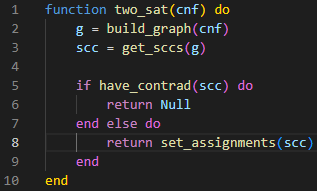
\includegraphics[width = 0.7\textwidth]{resources/code4.png}

            Para analizar la complejidad temporal del algoritmo se tienen en cuenta los siguientes aspectos:
            \begin{enumerate}
                \item Construcción del grafo: para construir el grafo es necesario recorrer la fórmula para hallar las variables
                (para crear los nodos) y crear las aristas. Esto tiene costo $O(|cnf|)$. Como por cada cláusulas existen solamente dos
                literales, entonces podemos decir que $|cnf| =  2m$, donde $m$ es la cantidad de cláusulas. Luego construir el grafo tiene costo
                $O(m)$. El grafo tendrá $2n$ nodos ($n$ es la cantidad de variables) y $2m$ aristas ($m$ es la cantidad de cláusulas).
                \item Hallar las componentes fuertemente conexas tiene costo $O(2n+2m) = O(n+m)$.
                \item Comprobar si existe una contradicción en las $SCC_s$ tiene costo $O(n)$ ya que para ello se realiza un recorrido por 
                los nodos y se puede comprobar en $O(1)$ si el opuesto de dicho nodo pertenece a la misma componente conexa. Esta comprobación 
                puede realizarse teniendo guardado en una estructura de datos donde indexar tenga costo $O(1)$ (diccionario o  array en caso que 
                las variables se traten con enteros) la $SCC$ a donde pertenezca cada nodo.
                \item Para construir las asignaciones es necesario recorrer los nodos de cada $SCC$ y se puede guardar en un array de tamaño $2n$
                el valor asigando a cada nodo. Si se tratan como enteros las variables esta indexación puede hacerse en $O(1)$, por lo que el costo 
                será $O(n)$.
            \end{enumerate} 
            Apoyándose en el análisis anterior se puede determinar que el algoritmo tiene complejidad temporal $O(n+m)$.           

    \subsection*{K-aproximación}
        
        La idea de este algoritmo es hacer una especie de algoritmo greedy con daños colaterales. 
        Por cada iteración del algoritmo se determina cual es el literal más frecuente en la fórmula que
        aun no tenga valor asignado. A ese literal se le asigna valor de verdad 1 y a su opuesto 0, esto convierte 
        todas las cláusulas donde se encuentre en verdaderas. Esta decisión tiene como efecto negativo 
        que cláusulas que contengan el opuesto de un literal con valor 1, potencialmente pueden resultar negativas.
        Pero como el literal escogido es el más frecuente, tendrá una ocurrencia mayor o igual a su opuesto, por tanto
        con esta elección de valor para esa variable se obtiene una cantidad de cláusulas verdaderas mayor o igual 
        a la cantidad de falsas. Esto implica que en el peor de los casos en cada iteración, la cantidad de cláusulas verdaderas
        sea la mitad del total de cláusulas evaluadas. Por tanto al finalizar el algoritmo
        al menos la mitad de las cláusulas son verdaderas.

        \begin{proof}
            El algoritmo termina ya que por cada iteración se elimina al menos una cláusula de la fórmula original, 
            y dicha fórmula es finita. 

            Correctitud:

            Sea $l_i$ el literal más frecuente en una iteración cualquiera del algoritmo y $-l_i$ su opuesto.
            Sea $cl_i$ la cantidad de cláusulas que se evaluaron como verdaderas en esta iteración y $cl_i^{-1}$ las que
            se evaluaron en falso. 
            
            Supongamos que $cl_i^{-1} > cl_i$, entonces la cantidad de cláusulas donde no aparece $l_i$ y si $-l_i$ 
            es mayor a la cantidad de cláusulas donde aparece $l_i$, lo cual es una contradicción ya que $l_i$ era el literal
            más frecuente. Por tanto $cl_i^{-1} \leq cl_i$.

            Como 
            \begin{align*}
                cl_1^{-1} \leq cl_1, cl_1^{-1} \leq cl_1, \dots, cl_m^{-1} \leq cl_m
            \end{align*}
            Entonces
            \begin{align*}
                cl_1^{-1} + cl_2^{-1} + \dots + cl_m^{-1} \leq cl_1 + cl_2 + \dots + cl_m
            \end{align*}
            Por tanto la cantidad total de cláusulas verdaderas es como mínimo la mitad del total de 
            cláusulas.
        \end{proof}
        Este algoritmo resulta ser una 2-Aproximación para el problema.

        \subsubsection*{Pseudocódigo}
            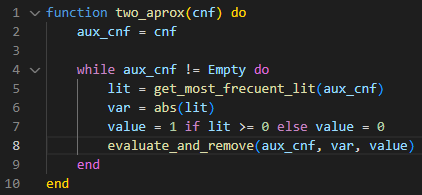
\includegraphics[width = 0.7\textwidth]{resources/code5.png}

            La complejidad temporal de este algoritmo está determina por la cantidad 
            de veces que se ejecuta el ciclo y el costo de las operaciones realizadas
            detro. 
            
            En cada iteración del ciclo al menos una cláusula es eliminada de la fórmula,
            por lo que a lo sumo se ejecutará $m$ veces, donde $m$ es la cantidad de cláusulas
            de la fórmula.

            Luego seleccionar el literal más frecuente tiene costo $O(|cnf|)$. Para ello
            puede realizarse un recorrido por $cnf$ contando las repeticiones de cada literal y 
            guardando el valor en un array. Las variables se toman como enteros para indexar en $O(1)$ 
            y sus negaciones ocuparán la posición $variable + len(variables)$, de modo que 
            el array tendrá tamaño $2*len(variables)$.
            Luego se recorre dicho array para seleccionar el literal más frecuente. Esto tiene
            costo $O(2*len(variables))$, como $len(variables) \leq |cnf|$, entonces tiene costo $O(|cnf|)$.

            Resta otorgar valor 1 al literal (0 a su opuesto) y eliminar las cláusulas en las que aparece. 
            En un recorrido por la fórmula se puede detectar las cláusulas que contienen al literal y se puede otorgar
            valor 0 a su opuesto, esto tiene complejidad $O(|cnf|)$. 
            Luego teniendo las cláusulas a eliminar, se puede construir una nueva fórmula que no contenga 
            dichas cláusulas, con complejidad $O(m)$. Entonces todo el proceso anterior tendrá
            costp $O(|cnf| + m)$, como $m \leq |cnf|$, el costo sería $O(|cnf|)$.
            
            Finalmente el algoritmo tiene complejidad temporal $O(m*|cnf|)$. 

\section*{Experimentación}
    Se generaron [PONER CUANTOS CASOS SE GENERARON] casos de prueba para analizar los resultados arrojasdos por cada 
    algoritmo, para así comprobar de manera práctica su efectividad. Los resultados fueron almacenados en archivos 
    $.json$ anexados junto al reporte.
    
    Una comparativa interesante resulta de comparar el algoritmo por fuerza bruta con el algoritmo DPLL. A 
    pesar de tener ambos la misma complejidad temporal, en la práctica DPLL tiene a tener mucha más eficiencia 
    que la fuerza bruta. 

    \includegraphics*[width = 0.9\textwidth]{resources/comp_algs.png}
    
    [EXPLICAR LAS GRÁFICAS]



\bibliography{ref}
\end{document}